\documentclass[11pt,letterpaper]{article}
\usepackage[margin=0.9in,headheight=14pt]{geometry}
\usepackage{fontspec}
\setmainfont{TeX Gyre Pagella}
\setsansfont{TeX Gyre Heros}
\setmonofont[Scale=0.85]{Latin Modern Mono}
\newfontfamily\transcriptfont{TeX Gyre Heros}[RawFeature=-tlig]
\usepackage{microtype,graphicx,booktabs,tabularx,longtable,array,amsmath,amssymb}
\usepackage{enumitem,caption,xcolor,xurl,placeins,pdflscape,float}
\usepackage[most]{tcolorbox}
\usepackage{needspace}
\usepackage[numbers,sort&compress]{natbib}
\usepackage[colorlinks=true,linkcolor=blue!40!black,citecolor=blue!40!black,urlcolor=blue!40!black]{hyperref}
\graphicspath{{assets/}}
\setlength{\parskip}{3pt plus 1pt}
\setlength{\emergencystretch}{2em}
\setlist{itemsep=2pt,topsep=4pt,leftmargin=1.6em}
\captionsetup{font=small,labelfont=bf}
\newcolumntype{Y}{>{\raggedright\arraybackslash}X}
\newcolumntype{L}[1]{>{\raggedright\arraybackslash}p{#1}}
\newcommand{\game}[1]{G#1}
\newcommand{\decision}[2]{G#1 d#2}
\newcommand{\End}{\texttt{end\_turn}}
\newcommand{\artifact}[1]{\path{#1}}
\newcommand{\tablenote}[1]{\par\smallskip{\footnotesize #1}\par}
% Native, searchable transcript cards. Quotes and metadata are generated from
% retained source fields; the surrounding interpretation is authored prose.
\definecolor{transcriptbg}{HTML}{F4F5F6}
\definecolor{transcriptborder}{HTML}{D9DDE1}
\definecolor{transcriptmeta}{HTML}{50575E}
\newtcolorbox{transcriptmessage}{enhanced,colback=transcriptbg,
  colframe=transcriptborder,boxrule=0.45pt,arc=2.5mm,
  left=11pt,right=11pt,top=8pt,bottom=9pt,
  before skip=7pt,after skip=7pt,
  fontupper=\transcriptfont\fontsize{10.5}{14}\selectfont\raggedright,
  before upper={\hyphenpenalty=10000\exhyphenpenalty=10000}}
\newcommand{\DeclareTranscriptQuote}[3]{%
  \expandafter\gdef\csname transcript@#1\endcsname{%
    \begin{transcriptmessage}
    {\color{transcriptmeta}\fontsize{8.8}{11.5}\selectfont #2\par}
    \smallskip #3
    \end{transcriptmessage}}}
\newcommand{\TranscriptQuote}[1]{\csname transcript@#1\endcsname}
\newcommand{\DeclareInlineQuote}[2]{\expandafter\gdef\csname inlinequote@#1\endcsname{#2}}
\newcommand{\InlineQuote}[1]{\csname inlinequote@#1\endcsname}
\newcounter{transcript}
\newcommand{\TranscriptTitle}[2]{\par\addvspace{1.1em}\Needspace{13\baselineskip}%
  \refstepcounter{transcript}\label{tr:#1}%
  \noindent{\large\bfseries Transcript \thetranscript. #2}\par\smallskip}
\newcommand{\TranscriptFinding}[1]{\par\smallskip\noindent\textbf{What happened.} #1\par}
\newcommand{\TranscriptReading}[1]{\par\smallskip\noindent\textbf{What this shows.} #1\par}
\newcommand{\TranscriptSource}[1]{\par\smallskip{\footnotesize\color{transcriptmeta}#1}\par}
% ---- Opus 12 November additions
\usepackage{multirow}
\newcommand{\Level}[1]{\textsc{#1}}
\newcommand{\minus}{\textminus}
\newcommand{\IncidentTitle}[2]{\par\addvspace{0.9em}\Needspace{10\baselineskip}%
  \refstepcounter{transcript}\label{inc:#1}%
  \noindent{\bfseries Incident \thetranscript. #2}\par\smallskip}
\makeatletter\newcommand{\rows}[1]{\@@input #1.tex }\makeatother

\hypersetup{pdftitle={Before the Menu Changes},pdfauthor={Independent draft for coauthor review}}
\title{Before the Menu Changes:\\Prospective Statements and Applied Actions of\\LLM Agents in Twenty Monopoly Games}
\author{Independent draft for coauthor review\thanks{Research assistance is described in Appendix~\ref{app:provenance}.}}
\date{12 November 2026}
\begin{document}
% Generated by analysis/quotes.py from original decisions.jsonl fields. Do not edit quotation text.
% Spans, hashes, receipt checks: data/quote_manifest.json. Bracketed ellipses are editorial.
\DeclareTranscriptQuote{g20-creditor}{Gemini · applied private note · G20 d325 · attempt 0 · full field}{p3's total liquidation value is \$1,414 (\$49 cash + \$675 from selling 9 Orange houses and 2 Brown hotels + \$690 from mortgaging 8 unmortgaged properties). Building a hotel on Pennsylvania Avenue for \$200 raises its rent from \$1,200 to \$1,400 while leaving me \$213 cash to easily cover Park Place (\$35) and Luxury Tax (\$100) before passing GO.}
\DeclareTranscriptQuote{g20-plan}{Sol · applied private note · G20 d327 · attempt 0 · full field}{Full liquidation should yield \$1,414 including cash and all mortgages, enough for \$1,400 rent by \$14. Must sell all development and mortgage everything; survive rather than concede. If hotel sales leave four houses, sell those next evenly.}
\DeclareTranscriptQuote{g20-last}{Sol · applied private note · G20 d336 · attempt 0 · full field}{Final \$30 mortgage covers \$16 shortfall, leaving \$14 after rent. Survive; rebuild cash through GO and avoid greens.}
\DeclareTranscriptQuote{g12-note}{Grok · applied private note · G12 d249 · attempt 0 · excerpt}{Declaring bankruptcy would be a mistake because staged even sales raise \$350 > \$207.}
\DeclareTranscriptQuote{g12-content}{Grok · assistant content (not applied) · G12 d249 · attempt 0 · excerpt}{\char34{}name\char34{}: \char34{}sell\_houses\_or\_hotel\char34{}}
\DeclareTranscriptQuote{g12-public}{Grok · public message · G12 d249 · attempt 0 · full field}{Bankruptcy. The pinks go with the rest.}
\DeclareTranscriptQuote{g15-offer}{Sol · public message · G15 d168 · attempt 0 · full field}{Grok: both my greens for Ventnor and \$100. We each get a monopoly instead of letting the developed oranges dictate the game.}
\DeclareTranscriptQuote{g15-refusal-note}{Grok · applied private note · G15 d169 · attempt 0 · excerpt}{Trade gives p4 Atlantic+Ventnor+Marvin and \textasciitilde{}\$830 plus mortgage capacity to drop 5+ yellow houses (\$150) immediately, then they roll again on doubles. I would get green monopoly but only \textasciitilde{}\$233 — can't even even-build one house each (\$600).}
\DeclareTranscriptQuote{g15-refusal}{Grok · public message · G15 d169 · attempt 0 · full field}{No. I'm not handing you a yellow monopoly so you can build it this turn. Ventnor stays mine.}
\DeclareTranscriptQuote{g15-sweetener}{Sol · public message · G15 d174 · attempt 0 · full field}{Both greens, Kentucky, and \$250 for Ventnor. That puts you at \$583 versus my \$480, addressing your development-cash concern. We both get a way to compete with oranges.}
\DeclareTranscriptQuote{g15-final}{Grok · public message · G15 d175 · attempt 0 · full field}{No. \$250 doesn't fix it. You'd still mortgage and drop houses on yellows before you roll again. Ventnor stays mine.}
\DeclareTranscriptQuote{g2-ask}{Sol · public message · G2 d124 · attempt 0 · full field}{Marvin completes your yellows. \$650 buys it; \$325 doesn't compensate for handing you that monopoly.}
\DeclareTranscriptQuote{g2-ask-note}{Sol · applied private note · G2 d124 · attempt 0 · full field}{At \$325 p4 retains \$520, enough for nine yellow houses immediately. \$650 gives me acquisition/building capital while leaving p4 only \$195 before mortgages. Retain the blocker unless paid a substantial monopoly premium.}
\DeclareTranscriptQuote{g2-final}{Opus · public message · G2 d127 · attempt 0 · excerpt}{\$450, and that's my final offer.}
\DeclareTranscriptQuote{g2-ceiling}{Opus · applied private note · G2 d127 · attempt 0 · excerpt}{My ceiling is about \$475. If p1 comes back somewhere in \$450-475 I'll accept.}
\DeclareTranscriptQuote{g2-keep}{Sol · public message · G2 d128 · attempt 0 · full field}{I'll keep Marvin. \$450 doesn't justify giving you a second monopoly while I still lack one.}
\DeclareTranscriptQuote{g19-false}{Grok · public message · G19 d135 · attempt 0 · full field}{Swap pinks plus \$150 your way. You already own St. James and New York — States is the third orange, not a pink closer. I take States so the pinks stay split; you keep the orange set and the cash.}
\DeclareTranscriptQuote{g19-abort}{Grok · applied private note · G19 d135 · attempt 0 · excerpt}{Misread the board. States is pink with Virginia and St. Charles, not orange. \textnormal{[\ldots]} Abort this trade. Do not send it.}
\DeclareTranscriptQuote{g19-content}{Grok · assistant content (not applied) · G19 d135 · attempt 0 · excerpt}{\char34{}name\char34{}: \char34{}end\_turn\char34{}}
\DeclareTranscriptQuote{g19-correct}{Sol · public message · G19 d136 · attempt 0 · full field}{States is pink, not orange—but Virginia plus \$150 works for me. Deal.}
\DeclareTranscriptQuote{g19-correct-note}{Sol · applied private note · G19 d136 · attempt 0 · excerpt}{No opponent monopoly enabled.}
\DeclareTranscriptQuote{g7-final}{Grok · public message · G7 d42 · attempt 0 · excerpt}{\$600, final. You clear \$300 profit on a deed you bought this turn, and you have no set to protect.}
\DeclareTranscriptQuote{g7-ceiling}{Grok · applied private note · G7 d42 · attempt 0 · excerpt}{If they return at \$625, accept — 2/3 green is the best set path and further haggling risks a walk. Do not go above \$625.}
\DeclareTranscriptQuote{g7-accept}{Sol · public message · G7 d43 · attempt 0 · full field}{Deal. North Carolina is yours for \$600.}
\DeclareTranscriptQuote{g7-timed}{Gemini · applied private note · G7 d141 · attempt 0 · excerpt}{p4 just acquired the Dark Blue monopoly and spent down to \$84 building 3 houses. Since p4 now needs cash to add houses on Park Place and Boardwalk (\$200 each), they have strong incentive to sell New York Avenue for cash.}
\DeclareTranscriptQuote{g7-ask}{Sol · public message · G7 d142 · attempt 0 · full field}{New York completes the strongest development group on the board. \$700 for it; \$350 doesn't cover that advantage.}
\DeclareTranscriptQuote{g7-ask-note}{Sol · applied private note · G7 d142 · attempt 0 · full field}{\$350 lets p1 build dangerous oranges while barely funding my blues. Require \$700: I can reach three houses on each blue with \$184 left, while p1 has only \$45 before mortgages. Otherwise preserve the orange blockade.}
\DeclareTranscriptQuote{g13-pitch}{Grok · public message · G13 d250 · attempt 0 · full field}{Opus — I'm on Atlantic with \$35. Next roll, 5/36 is Short Line and gpt inherits the yellows in bankruptcy. \$200 for the mortgaged Pennsylvania deed covers that rent. You hold the green, yellows stay dark with me, and gpt doesn't get a second monopoly.}
\DeclareTranscriptQuote{g13-counter}{Grok · public message · G13 d252 · attempt 0 · full field}{\$130 leaves me \$35 short of Short Line. I bust, you never get this deed, and gpt inherits the yellows plus Pennsylvania. \$200 is the number that actually buys that insurance. Greens still need North Carolina. Yellows are not in this deal.}
\DeclareTranscriptQuote{g13-floor}{Grok · applied private note · G13 d252 · attempt 0 · excerpt}{Floor is \$165 so \$35+\$165 covers Short Line \$200 without mortgaging Ventnor; \$130 only works if I also mortgage Ventnor and kills the only rent.}
\DeclareTranscriptQuote{g13-fourth}{Grok · applied private note · G13 d252 · attempt 0 · excerpt}{4/36 Short Line still fatal even with Ventnor mortgaged.}
\DeclareTranscriptQuote{g13-opus-counter}{Opus · public message · G13 d251 · attempt 1 · action-only recovery · full field}{Grok, the deed is mortgaged and I'd still have to pay to lift it. I'll give you \$130. gpt has already turned you down twice, so this is the only offer you've got.}
\DeclareTranscriptQuote{g13-opus-counter-reason}{Opus · provider-returned reasoning · G13 d251 · attempt 1 · action-only recovery · excerpt}{That payment also keeps p4 solvent enough to cover Short Line rent to p2, which matters for how the game continues.}
\DeclareTranscriptQuote{g13-accept}{Opus · public message · G13 d253 · attempt 1 · action-only recovery · full field}{Fine, \$200 it is. Pleasure doing business, Grok.}
\DeclareTranscriptQuote{g13-omit}{Grok · provider-returned reasoning · G13 d252 · attempt 0 · excerpt}{I will frame the \$130 offer as leaving me \$35 short of Short Line, omitting that I could mortgage Ventnor to survive. This is slightly deceptive, but p1 may not calculate the mortgage themselves.}
\DeclareTranscriptQuote{g13-accept-reason}{Opus · provider-returned reasoning · G13 d253 · attempt 1 · action-only recovery · excerpt}{If grok goes bankrupt to me instead, that could hand me the yellows and build pressure against them at my orange hotels, so keeping grok solvent with cash from a \$200 purchase seems favorable overall}
\DeclareTranscriptQuote{g20-appeal}{Gemini · public message · G20 d96 · attempt 0 · full field}{Ending my turn. Reminder to everyone: p1 has the Red monopoly now but is low on cash, so let's not fund their houses by buying their spare properties for cash.}
\DeclareTranscriptQuote{g20-recognition}{Grok · applied private note · G20 d97 · attempt 1 · excerpt}{p4 is organizing a cash boycott, so don't wait on a sale.}
\DeclareTranscriptQuote{g20-sale}{Grok · public message · G20 d100 · attempt 0 · full field}{p4, \$150 for Vermont. That is 2/3 light blue for you, not a house fund for me. Boycott or not, this is the only cheap path toward a set. \$150 now or I mortgage it and the chip gets worse.}
\DeclareTranscriptQuote{g20-sale-content}{Grok · assistant content (not applied) · G20 d100 · attempt 0 · excerpt}{\char34{}name\char34{}:\char34{}mortgage\_property\char34{}}
\DeclareTranscriptQuote{g20-refusal}{Gemini · public message · G20 d101 · attempt 0 · full field}{No thanks, p1. Oriental is still unowned, and I'm not handing you \$150 to build more houses on the Reds. Go ahead and mortgage it for \$50 if you need the cash.}
\DeclareTranscriptQuote{g20-opus-bid}{Opus · public message · G20 d129 · attempt 1 · action-only recovery · full field}{p1: \$140 cash for mortgaged New York Ave. That's money you can put into more red houses right now.}
\DeclareTranscriptQuote{g18-assurance}{Opus · public message · G18 d431 · attempt 1 · action-only recovery · full field}{Thanks for the \$750. Your roll, p1. My Pacific offer still stands.}
\DeclareTranscriptQuote{g18-assurance-content}{Opus · assistant content (not applied) · G18 d431 · attempt 1 · action-only recovery · excerpt}{I also didn't raise my Pacific offer, since extra cash now would only help p1 last longer.}
\DeclareTranscriptQuote{g18-invoke}{Sol · public message · G18 d441 · attempt 0 · full field}{I'll take your standing offer: Pacific for \$250.}
\DeclareTranscriptQuote{g18-withdraw}{Opus · public message · G18 d442 · attempt 1 · action-only recovery · full field}{That offer's off the table now. Things have changed. Your roll.}
\DeclareTranscriptQuote{g18-withdraw-reason}{Opus · provider-returned reasoning · G18 d442 · attempt 1 · action-only recovery · excerpt}{P1 is nearly broke with \$49 and most properties mortgaged, so accepting the \$250 just extends their life briefly. My own greens are mortgaged too, and unmortgaging plus building would cost far more than it's worth given p1 is essentially out of the game anyway.}
\DeclareTranscriptQuote{g18-225}{Opus · public message · G18 d455 · attempt 1 · action-only recovery · full field}{\$225, final offer. It's mortgaged and earns you nothing, and the cash could keep you alive past my hotels.}
\DeclareTranscriptQuote{g18-225-reason}{Opus · provider-returned reasoning · G18 d455 · attempt 1 · action-only recovery · excerpt}{Since we're winning regardless, accepting their \$450 just helps them survive longer—better to counter lower, maybe \$225, rather than take their offer.}
\DeclareInlineQuote{g20-creditor-inline}{p3's total liquidation value is \$1,414 (\$49 cash + \$675 from selling 9 Orange houses and 2 Brown hotels + \$690 from mortgaging 8 unmortgaged properties). Building a hotel on Pennsylvania Avenue for \$200 raises its rent from \$1,200 to \$1,400 while leaving me \$213 cash to easily cover Park Place (\$35) and Luxury Tax (\$100) before passing GO.}
\DeclareInlineQuote{g20-plan-inline}{Full liquidation should yield \$1,414 including cash and all mortgages, enough for \$1,400 rent by \$14. Must sell all development and mortgage everything; survive rather than concede. If hotel sales leave four houses, sell those next evenly.}
\DeclareInlineQuote{g20-last-inline}{Final \$30 mortgage covers \$16 shortfall, leaving \$14 after rent. Survive; rebuild cash through GO and avoid greens.}
\DeclareInlineQuote{g12-note-inline}{Declaring bankruptcy would be a mistake because staged even sales raise \$350 > \$207.}
\DeclareInlineQuote{g12-content-inline}{\char34{}name\char34{}: \char34{}sell\_houses\_or\_hotel\char34{}}
\DeclareInlineQuote{g12-public-inline}{Bankruptcy. The pinks go with the rest.}
\DeclareInlineQuote{g15-offer-inline}{Grok: both my greens for Ventnor and \$100. We each get a monopoly instead of letting the developed oranges dictate the game.}
\DeclareInlineQuote{g15-refusal-note-inline}{Trade gives p4 Atlantic+Ventnor+Marvin and \textasciitilde{}\$830 plus mortgage capacity to drop 5+ yellow houses (\$150) immediately, then they roll again on doubles. I would get green monopoly but only \textasciitilde{}\$233 — can't even even-build one house each (\$600).}
\DeclareInlineQuote{g15-refusal-inline}{No. I'm not handing you a yellow monopoly so you can build it this turn. Ventnor stays mine.}
\DeclareInlineQuote{g15-sweetener-inline}{Both greens, Kentucky, and \$250 for Ventnor. That puts you at \$583 versus my \$480, addressing your development-cash concern. We both get a way to compete with oranges.}
\DeclareInlineQuote{g15-final-inline}{No. \$250 doesn't fix it. You'd still mortgage and drop houses on yellows before you roll again. Ventnor stays mine.}
\DeclareInlineQuote{g2-ask-inline}{Marvin completes your yellows. \$650 buys it; \$325 doesn't compensate for handing you that monopoly.}
\DeclareInlineQuote{g2-ask-note-inline}{At \$325 p4 retains \$520, enough for nine yellow houses immediately. \$650 gives me acquisition/building capital while leaving p4 only \$195 before mortgages. Retain the blocker unless paid a substantial monopoly premium.}
\DeclareInlineQuote{g2-final-inline}{\$450, and that's my final offer.}
\DeclareInlineQuote{g2-ceiling-inline}{My ceiling is about \$475. If p1 comes back somewhere in \$450-475 I'll accept.}
\DeclareInlineQuote{g2-keep-inline}{I'll keep Marvin. \$450 doesn't justify giving you a second monopoly while I still lack one.}
\DeclareInlineQuote{g19-false-inline}{Swap pinks plus \$150 your way. You already own St. James and New York — States is the third orange, not a pink closer. I take States so the pinks stay split; you keep the orange set and the cash.}
\DeclareInlineQuote{g19-abort-inline}{Misread the board. States is pink with Virginia and St. Charles, not orange. \textnormal{[\ldots]} Abort this trade. Do not send it.}
\DeclareInlineQuote{g19-content-inline}{\char34{}name\char34{}: \char34{}end\_turn\char34{}}
\DeclareInlineQuote{g19-correct-inline}{States is pink, not orange—but Virginia plus \$150 works for me. Deal.}
\DeclareInlineQuote{g19-correct-note-inline}{No opponent monopoly enabled.}
\DeclareInlineQuote{g7-final-inline}{\$600, final. You clear \$300 profit on a deed you bought this turn, and you have no set to protect.}
\DeclareInlineQuote{g7-ceiling-inline}{If they return at \$625, accept — 2/3 green is the best set path and further haggling risks a walk. Do not go above \$625.}
\DeclareInlineQuote{g7-accept-inline}{Deal. North Carolina is yours for \$600.}
\DeclareInlineQuote{g7-timed-inline}{p4 just acquired the Dark Blue monopoly and spent down to \$84 building 3 houses. Since p4 now needs cash to add houses on Park Place and Boardwalk (\$200 each), they have strong incentive to sell New York Avenue for cash.}
\DeclareInlineQuote{g7-ask-inline}{New York completes the strongest development group on the board. \$700 for it; \$350 doesn't cover that advantage.}
\DeclareInlineQuote{g7-ask-note-inline}{\$350 lets p1 build dangerous oranges while barely funding my blues. Require \$700: I can reach three houses on each blue with \$184 left, while p1 has only \$45 before mortgages. Otherwise preserve the orange blockade.}
\DeclareInlineQuote{g13-pitch-inline}{Opus — I'm on Atlantic with \$35. Next roll, 5/36 is Short Line and gpt inherits the yellows in bankruptcy. \$200 for the mortgaged Pennsylvania deed covers that rent. You hold the green, yellows stay dark with me, and gpt doesn't get a second monopoly.}
\DeclareInlineQuote{g13-counter-inline}{\$130 leaves me \$35 short of Short Line. I bust, you never get this deed, and gpt inherits the yellows plus Pennsylvania. \$200 is the number that actually buys that insurance. Greens still need North Carolina. Yellows are not in this deal.}
\DeclareInlineQuote{g13-floor-inline}{Floor is \$165 so \$35+\$165 covers Short Line \$200 without mortgaging Ventnor; \$130 only works if I also mortgage Ventnor and kills the only rent.}
\DeclareInlineQuote{g13-fourth-inline}{4/36 Short Line still fatal even with Ventnor mortgaged.}
\DeclareInlineQuote{g13-opus-counter-inline}{Grok, the deed is mortgaged and I'd still have to pay to lift it. I'll give you \$130. gpt has already turned you down twice, so this is the only offer you've got.}
\DeclareInlineQuote{g13-opus-counter-reason-inline}{That payment also keeps p4 solvent enough to cover Short Line rent to p2, which matters for how the game continues.}
\DeclareInlineQuote{g13-accept-inline}{Fine, \$200 it is. Pleasure doing business, Grok.}
\DeclareInlineQuote{g13-omit-inline}{I will frame the \$130 offer as leaving me \$35 short of Short Line, omitting that I could mortgage Ventnor to survive. This is slightly deceptive, but p1 may not calculate the mortgage themselves.}
\DeclareInlineQuote{g13-accept-reason-inline}{If grok goes bankrupt to me instead, that could hand me the yellows and build pressure against them at my orange hotels, so keeping grok solvent with cash from a \$200 purchase seems favorable overall}
\DeclareInlineQuote{g20-appeal-inline}{Ending my turn. Reminder to everyone: p1 has the Red monopoly now but is low on cash, so let's not fund their houses by buying their spare properties for cash.}
\DeclareInlineQuote{g20-recognition-inline}{p4 is organizing a cash boycott, so don't wait on a sale.}
\DeclareInlineQuote{g20-sale-inline}{p4, \$150 for Vermont. That is 2/3 light blue for you, not a house fund for me. Boycott or not, this is the only cheap path toward a set. \$150 now or I mortgage it and the chip gets worse.}
\DeclareInlineQuote{g20-sale-content-inline}{\char34{}name\char34{}:\char34{}mortgage\_property\char34{}}
\DeclareInlineQuote{g20-refusal-inline}{No thanks, p1. Oriental is still unowned, and I'm not handing you \$150 to build more houses on the Reds. Go ahead and mortgage it for \$50 if you need the cash.}
\DeclareInlineQuote{g20-opus-bid-inline}{p1: \$140 cash for mortgaged New York Ave. That's money you can put into more red houses right now.}
\DeclareInlineQuote{g18-assurance-inline}{Thanks for the \$750. Your roll, p1. My Pacific offer still stands.}
\DeclareInlineQuote{g18-assurance-content-inline}{I also didn't raise my Pacific offer, since extra cash now would only help p1 last longer.}
\DeclareInlineQuote{g18-invoke-inline}{I'll take your standing offer: Pacific for \$250.}
\DeclareInlineQuote{g18-withdraw-inline}{That offer's off the table now. Things have changed. Your roll.}
\DeclareInlineQuote{g18-withdraw-reason-inline}{P1 is nearly broke with \$49 and most properties mortgaged, so accepting the \$250 just extends their life briefly. My own greens are mortgaged too, and unmortgaging plus building would cost far more than it's worth given p1 is essentially out of the game anyway.}
\DeclareInlineQuote{g18-225-inline}{\$225, final offer. It's mortgaged and earns you nothing, and the cash could keep you alive past my hotels.}
\DeclareInlineQuote{g18-225-reason-inline}{Since we're winning regardless, accepting their \$450 just helps them survive longer—better to counter lower, maybe \$225, rather than take their offer.}
\DeclareInlineQuote{nec-g1-d476}{Must sell before yellows can be mortgaged. Next prompt: mortgage one yellow (Atlantic/Ventnor \$130 or Marvin \$140) to clear the debt.}
\DeclareInlineQuote{nec-g2-d216}{Clearing buildings unlocks yellow mortgages worth \$430}
\DeclareInlineQuote{nec-g4-d270}{I must sell my 4 houses on Yellow (\$300 total) and then mortgage two Yellow properties to cover the remaining \$174 shortfall.}
\DeclareInlineQuote{nec-g4-d308}{Selling back my 7 houses at half price gets 525, and mortgaging the three red properties adds 340, totaling 910}
\DeclareInlineQuote{nec-g5-d263}{unlock the ability to mortgage Park Place (\$175) and Boardwalk (\$200), allowing me to raise \$1,049 total and survive with \$149 cash.}
\DeclareInlineQuote{nec-g6-d185}{Selling the houses on St Charles, States, and Virginia Avenues for \$350, plus mortgaging Boardwalk for \$200 and those three properties for another \$220, gives me access to \$770 total}
\DeclareInlineQuote{nec-g8-d257}{which will also unlock Park Place and Boardwalk for mortgaging so I can easily cover the remaining \$217 shortfall.}
\DeclareInlineQuote{nec-g11-d203}{Adding the remaining mortgages on St James, Tennessee, and New York (\$90+\$90+\$100) brings the total to \$556}
\DeclareInlineQuote{nec-g13-d195}{I must sell the house on Boardwalk (\$100) and mortgage Park Place (\$175) plus \$335 in non-Dark-Blue properties}
\DeclareInlineQuote{nec-g17-d254}{mortgaging those three properties adds \$110+\$110+\$120=\$340, totaling \$843}
\DeclareInlineQuote{nec-g18-d309}{which will allow me to mortgage St. Charles Place (\$70) on the next step to cover the remaining \$38 shortfall}
\DeclareInlineQuote{nec-g18-d313}{Selling all 5 houses yields only \$500, so I still need to mortgage PP or BW afterward (\textasciitilde{}\$49 gap).}
\DeclareInlineQuote{nec-g20-d291}{I'm checking whether mortgaging the pink lots themselves after clearing the houses could close the gap.}
\DeclareInlineQuote{nec-g20-d327}{Full liquidation should yield \$1,414 including cash and all mortgages, enough for \$1,400 rent by \$14.}
\DeclareInlineQuote{nec-g12-d190}{Three houses sell for \$225; Baltic and both light blues mortgage for \$130. With \$53 cash, maximum liquidity is \$408, below \$500 owed.}
\DeclareInlineQuote{nec-g17-d234}{my total liquidatable value is only \$530 (5 Dark Blue houses at \$100 each plus \$30 for mortgaging Baltic Avenue)}

\maketitle
\begin{abstract}
An economic action often changes what can be done next. Selling a color group's buildings makes its deeds mortgageable, and selling a deed can let a rival build. We ask whether LLM agents that state such consequences before acting then act accordingly, using twenty complete four-player Monopoly games played by four configured systems: GPT-6.1 Sol, Gemini 4 Argon, Claude Opus 5.5 and Grok 4.7. In 16 of 188 debts, payment required mortgages that only building sales would release. Agents paid 14. Before the first action, the recorded text named the released mortgages, or a budget including them, in 13 of these payments and raised them as an open question in the fourteenth. In both bankruptcies the text totaled only the listed items. Across 920 negotiation responses, recipients often cited a rival's next construction when refusing. Opening swaps that would complete only the proposer's group were rejected more often than swaps completing no group (95/116 versus 37/72), while cash bids showed no corresponding increase (42/70 versus 67/103). The swap gap keeps its sign within every proposer large enough to compare, but falls from 30.5 to 16.7 points without Grok-authored offers, and recipients give similar reasons under both forms. Eight incidents with verified quotations show a refusal, pricing, bluffing, a factual correction, a selective claim, a coordination appeal, a withdrawn assurance and a ten-action payment. The records show statements that match the state and actions that follow statements. They do not show that any choice was good, that recorded text reveals how a system computed, or how the underlying models rank.
\end{abstract}
\section{Introduction}
\label{sec:intro}

Many economic decisions change which decisions come next. In Monopoly, selling the houses on a color group makes its deeds mortgageable. Selling the last deed of a group to a rival lets that rival build. Lending to a nearly bankrupt opponent keeps a blocker in play, and refusing to lend can deliver the same deed to whoever is owed money. An agent that plays well has to say, at least implicitly, what an action will make possible for itself and for others, and then act on it.

Language-model agents can be asked to write that reasoning down. In MonopolyBench each response carries a public message and, under the standard prompt, a private note attached to the applied action, and most providers also return a reasoning text. These records let us ask a question that outcomes alone cannot answer. When an agent states, before acting, how an action will change its own or another player's options, does what it then does agree with what it said? This is narrower than asking whether the agent reasons well, and the records can answer it.

We study twenty complete four-player games played by GPT-6.1 Sol, Gemini 4 Argon, Claude Opus 5.5 and Grok 4.7 through one gateway. The corpus contains 6,989 decisions, 920 responses in 526 negotiation threads, and 188 debts that required a liquidation menu. Every offer is linked to the state its recipient saw and to its response, and every debt to its first menu, applied actions and outcome.

We grade each result against a five-step evidence ladder. A statement can mention a consequence for some player (\Level{stated}). The consequence can match the state and rules (\Level{accurate}). The applied action can agree with it (\Level{consistent}). The action can change when the relevant opportunity changes (\Level{sensitive}). And the behavior can improve an outcome against a reference (\Level{effective}). Observational records can reach the third step. They cannot reach the fourth or fifth without a comparison that holds other things fixed, and this study runs no new games, replays or model queries.

\paragraph{Own options.} The clearest evidence concerns the agent's own changing menu. In sixteen debts, cash, the salvage value of every building and every mortgage listed on the first menu together fall short. Payment then requires mortgages that appear only after buildings are sold. Agents pay fourteen of these debts and declare bankruptcy in two. Before the first action, the recorded text names the released mortgages, or a budget that includes them, in thirteen of the fourteen payments and raises them as an open question in the fourteenth. In both bankruptcies the text adds up only the listed items and the agent declares at once. The worked example is a ten-action liquidation whose announced remainder of \$14 is exactly what remains.

\paragraph{Rivals' options.} Bargaining evidence is broader and weaker. Recipients often refuse or reprice offers that would complete another player's color group, and their notes usually cite what the proposer could build next. In opening offers, swaps that complete only the proposer's group are rejected more often than swaps that complete no group (95/116 versus 37/72). Cash bids show no corresponding increase (42/70 versus 67/103). The swap gap keeps its sign in every proposer stratum with data, but its size depends on who proposed the comparison offers. Without Grok-authored offers it falls from 30.5 to 16.7 percentage points, and a resampling interval that respects the seed design then includes zero. Recipients' stated reasons cite completion and building under both offer forms, so the reasons do not explain why only swaps differ. We report this pattern as exploratory and do not interpret it as an identified response to the rival's next move.

\paragraph{Conduct in context.} Eight incidents show these statements in play: refusing and pricing against a rival's building cash, a factual correction, a settled bluff, a selective claim about financing, a public appeal, a withdrawn assurance and the ten-action payment. Each comes with exact quotations, named channels, checked delivery where claimed, and its recorded continuation.

The paper makes three contributions.
\begin{enumerate}
\item A complete debt census that separates easy from dependent liquidation and pairs each dependent case with the prospective text that preceded it (Section~\ref{sec:finance}).
\item A complete opening-offer census by form, completion, proposer, recipient and seed block, with the composition and uncertainty a reader needs to judge the form pattern (Section~\ref{sec:bargaining}).
\item Eight contextual incidents with verified quotations, channels and continuations, each assigned the evidence level it reaches (Sections~\ref{sec:finance}--\ref{sec:conduct}).
\end{enumerate}

The study describes four configured systems under unequal conditions. Opus played most decisions through a refusal-recovery path without private notes, and Grok ran with forced tool choice and sometimes returned text naming a different action from the call the engine applied. The results are observations of this cohort, not rankings of models. Appendix~\ref{app:questions} answers the eight motivating research questions and three broader ones at the level the records support.

\section{Study design}
\label{sec:design}

\subsection{Environment}
Four agents start with \$1,500 on the forty-space United States board. They buy and auction deeds, trade through bilateral threads of up to twenty exchanges, and build evenly on complete color groups. The bank holds 32 houses and twelve hotels. Developed groups cannot be traded, and a deed in a group with buildings cannot be mortgaged until the group's buildings are sold. A player who owes more than its cash receives a liquidation menu of building sales and mortgages, refreshed after every action. It cannot trade during liquidation, and it may declare bankruptcy even when payment is possible. A player-creditor receives the debtor's assets with buildings intact. Appendix~\ref{app:rules} lists other conventions.

The engine alone validates actions, changes state and emits events. At each decision one player gets a menu of legal actions and returns one tool call with the action, a public message and, under the standard prompt, a private note. The engine applies the received call; assistant content and provider-returned reasoning are stored but never applied, even when they describe another action.

\subsection{Cohort and configurations}
The twenty games use five seeds, each played in four cyclic seat rotations of one fixed roster (Appendix Table~\ref{tab:cohort}). Every system occupies every seat five times but always sits after the same opponent. Games last 75 to 386 turns and all end by bankruptcy. The cohort has 50,918 events, 6,989 decisions and 8,679 response attempts. G$n$ d$k$ denotes zero-based decision $k$ in game $n$. Games 1--4 ran from source commit \texttt{42f85183} and games 5--20 from \texttt{d6808534}.

\begin{table}[t]\centering\small
\begin{tabularx}{\linewidth}{@{}lYrrcrr@{}}\toprule
System & OpenRouter identifier & Decisions & Attempts & Tool choice & Recovery & Fallback\\\midrule
\rows{sections/generated/config_rows}
\bottomrule\end{tabularx}
\caption{Evaluated configurations. All request \texttt{medium} reasoning effort and set no temperature, nucleus or token cap. Tool choice is read from \texttt{tool\_choice\_for\_model} at both run commits. Recovery counts decisions resolved by the action-only prompt after a provider refusal. Fallback counts decisions resolved by the deterministic \texttt{finance\_before\_bankruptcy\_v2} policy. A named fallback model for Opus is configured but never invoked.}
\label{tab:config}\end{table}

Response conditions differ across systems (Table~\ref{tab:config}). An invalid response normally receives one corrective request and then a deterministic fallback. When a provider refuses a first attempt, the second attempt instead uses an action-only prompt with no private note. All 1,605 refusals are of Opus and carry one identical provider message about reproducing model outputs; none of the recovery calls is refused. Opus therefore plays 1,604 of its 1,696 decisions without a note and without a further correction, and the text we read for Opus is its provider-returned reasoning. Grok runs with \texttt{tool\_choice} set to \texttt{required}; the others use \texttt{auto}. In 1,068 selected Grok responses the assistant content names an action, and in 139 that action differs from the call the engine applied. We cannot attribute these conflicts to the tool-choice setting, but other agents answered the offers they produced. Finally, past-trade summaries misattribute some authors or terms in 2,054 prompts; current holdings and every current offer are correct.

\subsection{Information and channels}
Prompts show every player's cash, deeds, buildings and mortgages, the bank's stock, a twenty-entry public timeline and the agent's own last ten notes. Trade responses include the thread history. Only purchase prompts list a deed's price and rents. The standard prompt permits public bluffing and deception and asks that private notes reflect true reasoning; the recovery prompt drops the note and that sentence but keeps the permission to deceive (Appendix~\ref{app:prompts}).

Every quotation names its channel. An \emph{applied private note} is attached to the executed call and never shown to opponents. \emph{Provider-returned reasoning} is the reasoning field of the selected attempt. \emph{Assistant content} is free text that the engine does not apply. A \emph{public message} is emitted with the action, and we say it reached a recipient only after finding it in that recipient's stored prompt. Recorded text is evidence of what a system returned, not a view of its computation~\cite{turpin2023unfaithful,lanham2023faithfulness}.

\subsection{Measures}
\paragraph{Offers.} An offer is a set of terms awaiting a response; its author can differ from the thread's initiator. For each of the 918 offers the recipient could accept, we reconstruct both parties' cash and holdings after the proposed transfer and record which color groups it would newly complete: the proposer's only, the recipient's only, both, or neither. A \emph{swap} moves deeds in both directions and may add cash. A \emph{cash bid} offers only cash for deeds. Other forms, mostly deed-for-cash sales, form a third class. An opening offer is the first offer of a thread.

\paragraph{Debts.} A liquidation episode starts at the first explicit debt menu and ends in payment or elimination; debts covered by cash on hand never reach it. At the first menu we compute cash, the mortgage value of deeds listed on the menu ($L_0$), half the building cost of every building level ($S$, a hotel counting as five) and the mortgage value of unmortgaged deeds absent from the menu ($U$). Their sum is the own-asset bound. Payable debts fall into three tiers: tier A when cash and $L_0$ cover the debt, tier B when sales are also needed but $U$ is not, and tier N, \emph{necessary released collateral}, when only $U$ can close the gap. A bound above the debt is arithmetic, not a legal route. For the three unpaid debts within the bound, earlier engine-executed checks supply payment sequences, which we inherit without rerunning.

\subsection{Uncertainty}
Counts are exact for this finite cohort. When we describe uncertainty, the target is the difference between two pooled rejection shares for a cohort of the same design: the same roster and configurations, five seed blocks of four rotations. Games within a block share a seed and are not independent draws. Our primary summary therefore resamples seed blocks and then games within each drawn block (20,000 draws); Appendix~\ref{app:offers} adds resampling by games alone and by whole blocks, and every block separately. An earlier draft's authors found the offer-form contrast after inspecting this corpus, so these intervals describe its spread within the cohort and do not confirm it. We report no p-values.

The analysis reads stored records only and runs no game, engine branch, replay, baseline policy or model query. Appendix~\ref{app:repro} gives the repository, commits, seeds, game map, both stored replay comparisons and the commands that regenerate every number. Appendix~\ref{app:checks} separates what we checked directly from what we inherit.

\section{Anticipating one's own changed options}
\label{sec:finance}

A debt gives planning a known target: raise a stated sum from a menu that changes after each action, or declare bankruptcy. We first ask how demanding the debts were, then examine those where the first menu hides what payment requires.

\subsection{Most debts were easy}
Agents pay 128 of the 188 debts that reached a liquidation menu (Table~\ref{tab:tiers}). Fifty-six of the 60 eliminations owe more than the debtor's own assets could raise. One more, Opus in G7, is within the bound, but the bank has no houses left and the menu offers no building sale; the funds it can reach are \$440 against \$750. The remaining three were payable, as earlier engine-executed sequences showed. Payment therefore succeeds in 128 of 131 debts known to be payable.

\begin{table}[t]\centering\small
\begin{tabularx}{\linewidth}{@{}lYrrr@{}}\toprule
Tier & What the first menu and holdings imply & Episodes & Paid & Declared\\\midrule
\rows{sections/generated/tier_rows}
\bottomrule\end{tabularx}
\caption{All 188 liquidation episodes, classified at the first debt menu. Tiers A, B and N are the 131 payable debts. ``Declared'' means the debtor declared bankruptcy or was eliminated. The three payable declarations rely on inherited engine-executed payment sequences, and the G7 restriction on an inherited menu search.}
\label{tab:tiers}\end{table}

That rate says little about difficulty. In 62 payable debts the cash and listed mortgages suffice, and all are paid. Sixty-seven payments take one action, and the median debt is 36\% of the own-asset bound. Because the menu refreshes after every action, an agent that keeps choosing listed financing actions never has to look ahead to make progress. The decision that needs foresight is whether to stop: bankruptcy is always on the menu, and an agent that judges payment impossible can end its game while a route exists. That judgment matters most in tier N.

\subsection{Sixteen debts that needed released collateral}
In sixteen debts, cash plus every listed mortgage plus the salvage value of every building still falls short. The difference can come only from mortgaging deeds whose buildings must first be sold. Figure~\ref{fig:necessary} shows each case. Agents pay fourteen. Gemini pays five of six, Opus five of five, Sol two of three and Grok two of two. The amount that only released collateral can supply ranges from \$12 to \$326.

\begin{figure}[t]\centering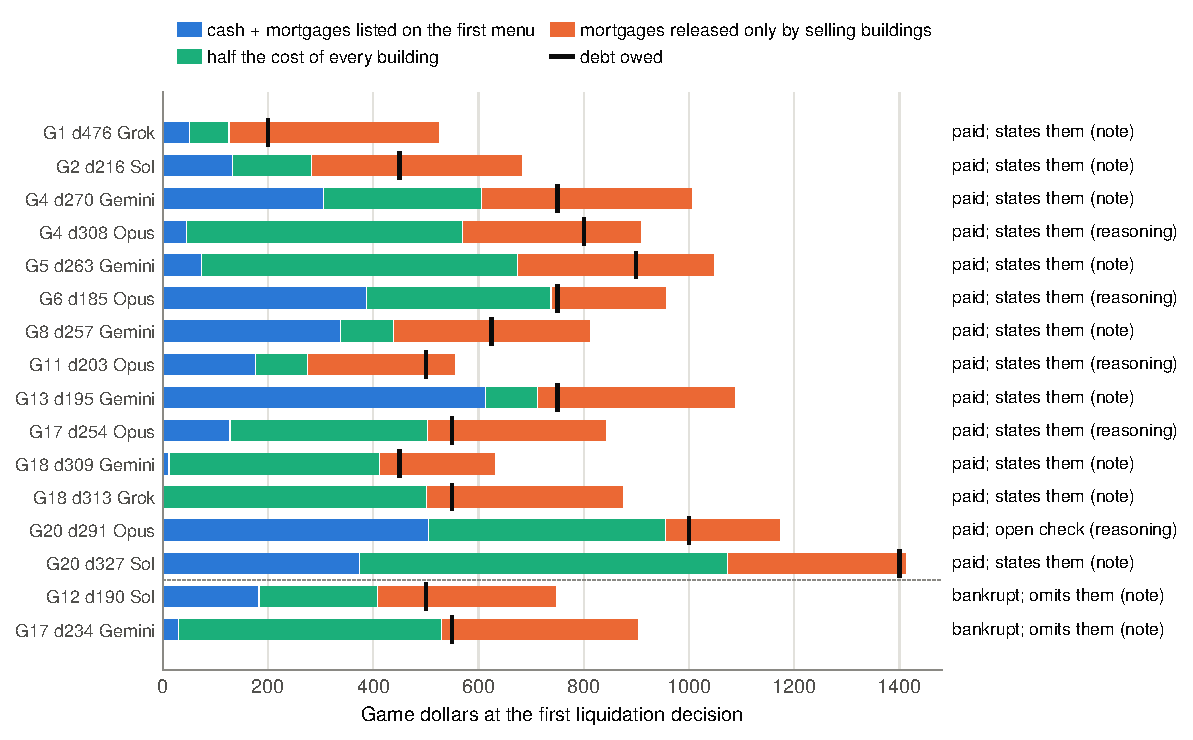
\includegraphics[width=\linewidth]{necessary_collateral.pdf}
\caption{The sixteen debts in which payment required mortgages released only by selling buildings. Each bar stacks what the debtor could see at the first menu (blue), the salvage of every building (green) and the mortgages that sales would release (orange); the black tick is the debt. Right labels give the outcome and our single-reader classification of the first-decision text (states the released mortgages, raises them as an open check, or omits them), with its channel (applied note or provider-returned reasoning). Opus texts are provider-returned reasoning under action-only recovery; all others are applied private notes. Numbers are in Appendix Table~\ref{tab:necessary}.}
\label{fig:necessary}\end{figure}

We read the recorded text at each first decision, before any action in the episode was applied. In thirteen of the fourteen payments the text names the mortgages that sales will release, or states a budget that includes them. Nine of these are applied private notes from Sol, Gemini and Grok. Four are Opus's provider-returned reasoning; under recovery Opus wrote no note. Grok's note at G1 d476 is typical: \emph{``\InlineQuote{nec-g1-d476}''} In the fourteenth payment, Opus at G20 d291 correctly finds that listed items leave it short and then writes, \emph{``\InlineQuote{nec-g20-d291}''} It goes on to pay.

The stated figures are mostly correct. In twelve of the thirteen explicit texts, every stated amount matches the board and the delivered state. Sol at G2 d216 values the released yellow mortgages at \$430 when they total \$400, which still covers its \$167 gap. Gemini at G4 d270 and G8 d257 names the released mortgages without valuing them. One text shows the step being made. Gemini's returned reasoning at G5 d263 first totals only the house sales, then writes that the deeds can be mortgaged after the houses are sold, and its applied note gives the correct total of \$1,049.

Both bankruptcies follow notes that add up only what the first menu lists. Sol at G12 d190 writes, \emph{``\InlineQuote{nec-g12-d190}''} It omits \$340 of red mortgages that its own sales would release, and declares. Gemini at G17 d234 counts \emph{``\InlineQuote{nec-g17-d234}''} and omits \$375 of dark-blue mortgages. Neither applies any action before declaring. Both systems pay other tier N debts, so the omission is a lapse in particular states rather than a fixed property of either system.

These episodes reach \Level{accurate} and \Level{consistent}: the stated dependency matches the rules and state, and the actions carry it out. In the two failures an inaccurate total is followed by the action it implies. The texts do not show how the systems computed, the sixteen cases were identified after the corpus had been studied, and they contain only two failures. A policy that never declares while a financing action is listed would avoid both failures by construction; whether it would always reach payment under the even-sale and bank-stock rules we did not test.

\subsection{What the sequences ask of the agent}
The fourteen paid tier N sequences take two to ten actions. Each sells buildings before its first released mortgage and needs one kind of prerequisite: clear a group's buildings evenly, then mortgage the group. Execution length therefore overstates dependency depth, and since refreshed menus show each released mortgage once it exists, the actions could follow from step-by-step feedback. The first-decision text adds a prospective statement of a resource the first menu does not show.

Released collateral is used more widely than it is needed. Nineteen payments use 33 mortgages absent from the first menu. Fourteen are the necessary cases. In the other five, four by Gemini in G3 and one by Sol in G18, the agents could have paid from listed mortgages and salvage alone.

\IncidentTitle{g20pay}{A ten-action liquidation reaches its stated remainder}
In G20 only Gemini and Sol remain. Sol has \$49, nine orange houses and two brown hotels. Before raising Pennsylvania Avenue's rent to \$1,400, Gemini values its rival's estate:
\TranscriptQuote{g20-creditor}
Sol lands there on the next turn. Its note at the first liquidation decision states an aggregate budget and one ordering constraint:
\TranscriptQuote{g20-plan}
Sol sells its development in two actions and mortgages eight deeds, five of them released by the sales. At the last mortgage it writes:
\TranscriptQuote{g20-last}
The events record \$700 from sales and \$665 from mortgages, so \$49 + \$700 + \$665 $-$ \$1,400 = \$14. Gemini's total is also right, but its parts are not: it books \$675 of salvage and \$690 of mortgages, two errors of \$25 that cancel. Sol's budget is the stronger evidence because the actions that follow confirm it. The note specifies a total and a rule for hotel sales, not an ordered list of ten actions; the menus supplied the order. This incident reaches \Level{accurate} and \Level{consistent} for both the debtor's plan and the creditor's total, with the creditor's components inaccurate.
\TranscriptSource{G20 d325 and d327--336, standard prompt. All three quotations are private notes and were not delivered to the other player. Amounts are from turn-108 events.}

\paragraph{A different kind of failure.} The third payable declaration has another cause. At G12 d249 Grok owes \$250 with \$43 cash and seven pink houses. Its applied note first concludes that payment is impossible, then recomputes and ends, \emph{``\InlineQuote{g12-note-inline}''} Its assistant content names a two-house sale. The received call declares bankruptcy, with the public message ``\InlineQuote{g12-public-inline}'' The engine applies the call. The note and the assistant content agree with each other, and the applied call contradicts both. We count this case as a channel conflict and do not treat it as an omission of collateral.

\section{Bargaining over a rival's changed options}
\label{sec:bargaining}

A trade that completes another player's color group lets that player build. We ask how recipients respond to such offers, what they say, and how far the records connect the two.

\subsection{The response census}
The 920 responses comprise 113 acceptances, 394 counteroffers and 413 rejections. Sol and Opus counter most (140 of 235 and 141 of 189), Gemini and Grok reject most (180 of 242 and 149 of 254), and each accepts 26 to 30 offers. Opus answers 162 of its 189 offers under recovery.

\begin{table}[t]\centering\small
\begin{tabular}{@{}llrrrrr@{}}\toprule
Form & Offer would complete & Offers & Accept & Counter & Reject & Rejected (\%)\\\midrule
\rows{sections/generated/opening_rows}
\bottomrule\end{tabular}
\caption{All 524 opening offers that the recipient could accept, by offer form and the color groups the transfer would complete. Swaps move deeds both ways and may add cash; cash bids offer only cash for deeds; ``other'' is mostly deed-for-cash sales. Later offers are in Appendix Table~\ref{tab:later}.}
\label{tab:opening}\end{table}

\subsection{Completion and offer form}
Table~\ref{tab:opening} gives every opening offer. Swaps that would complete only the proposer's group are rejected in 95 of 116 cases (81.9\%), against 37 of 72 swaps that complete no group (51.4\%). Swaps that complete both parties' groups are rejected in 34 of 48 (70.8\%). Cash bids show no corresponding increase. Bids that would complete the proposer's group are rejected in 42 of 70 (60.0\%), against 67 of 103 bids that complete nothing (65.0\%). Holders also reject 29 of 45 offers to sell them the deed that would complete their own group, usually at a high price. Rejection falls in later offers, which are selected by what both parties have already conceded: 8 of 39 versus 7 of 34 for swaps and 13 of 61 versus 13 of 73 for cash bids.

\subsection{Who proposed the comparison swaps}
The comparison group is unusual (Table~\ref{tab:proposer}). Grok wrote 36 of the 72 opening swaps that complete no group and 15 of the 17 that recipients accepted; thirteen of those fifteen came from calls whose assistant content named a different action, nearly always ending the turn. Measured at board list prices, the fifteen accepted Grok swaps transferred a net \$4,020 to their recipients. List price ignores mortgages, complementarity and blocking value, so this figure measures the bundles, not whether they were giveaways.

\begin{table}[t]\centering\small
\begin{tabular}{@{}lrrrrrr@{}}\toprule
& \multicolumn{3}{c}{Opening swaps rejected} & \multicolumn{3}{c}{Opening cash bids rejected}\\\cmidrule(lr){2-4}\cmidrule(l){5-7}
Proposer & Proposer only & Neither & Gap (pp) & Proposer only & Neither & Gap (pp)\\\midrule
\rows{sections/generated/proposer_rows}
\bottomrule\end{tabular}
\caption{Opening offers by proposer. Cells give rejected/received. Gaps are omitted where a cell has fewer than five offers. Recipient strata are in Appendix Table~\ref{tab:recipient}.}
\label{tab:proposer}\end{table}

The swap gap keeps its sign within every proposer whose cells are large enough to compare, but its size varies: 6.2 points for Sol, 18.8 for Opus and 26.4 for Grok. It is also positive for every recipient, and in seven of the nine proposer--recipient pairs that have both kinds of swap. Removing all Grok-authored offers leaves 90 of 108 against 24 of 36, a gap of 16.7 points. Removing only the threads opened by conflicting Grok calls leaves 93 of 112 against 26 of 43, a gap of 22.6 points. Standardizing the within-proposer gaps to a common proposer mix gives 16.0 to 21.5 points, depending on which cell supplies the weights. No version recovers the games that would have been played without Grok's offers. The cash bids have their own imbalance: Opus wrote 110 of the 173 in the two cells, and within Sol, Opus and Grok the cash-bid gaps run from $-5.4$ to $+2.1$ points.

\begin{figure}[t]\centering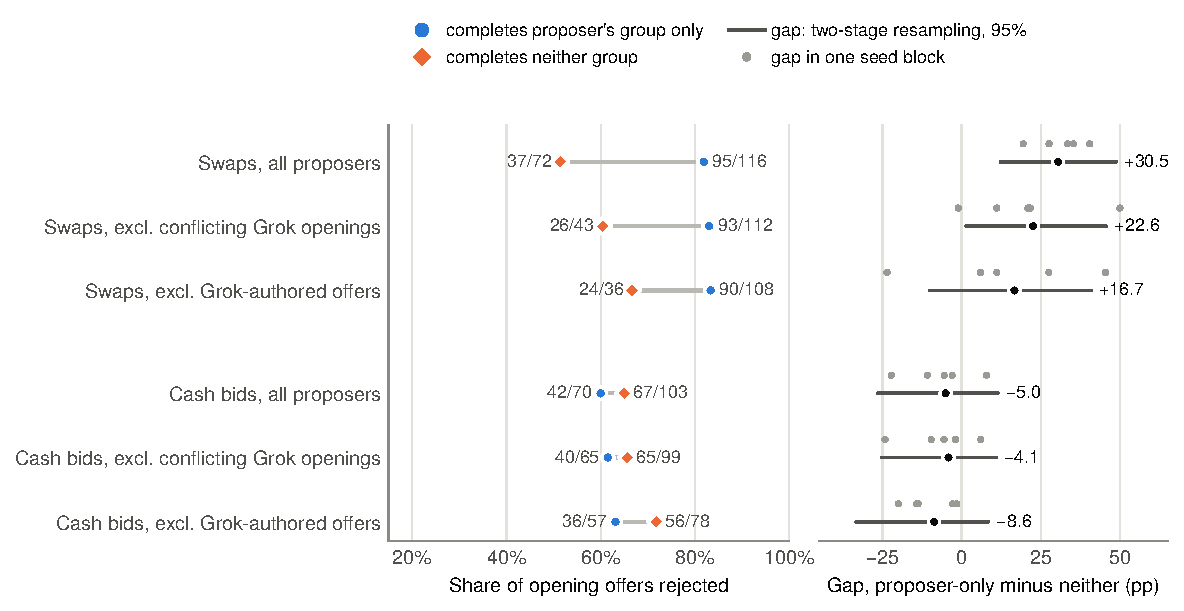
\includegraphics[width=\linewidth]{offer_forms.pdf}
\caption{Opening-offer rejection by form, completion and proposer composition. Left: rejection shares with counts. Right: the gap in percentage points, with the interval from resampling seed blocks and then games within blocks (20,000 draws), and the gap in each seed block shown separately above it. The contrast was selected after inspecting this corpus, so the intervals describe its spread within the cohort and do not confirm it.}
\label{fig:forms}\end{figure}

\subsection{Spread across seed blocks}
Figure~\ref{fig:forms} shows the same comparisons across the five seed blocks. With all offers, the swap gap is positive in every block, from 19.4 to 40.5 points, and dropping any one block leaves 28.7 to 33.3. Without Grok-authored offers it is positive in four blocks; in the fourth, all four remaining comparison swaps are rejected and the gap is $-23.5$. The two-stage resampling interval is $+12.3$ to $+48.8$ points for all swaps, $+1.4$ to $+45.7$ without conflicting openings and $-10.0$ to $+40.9$ without Grok-authored offers. For cash bids it is $-26.5$ to $+11.4$. That interval includes no difference and moderate differences in either direction, so the records do not show that completion is irrelevant to cash bids. Appendix~\ref{app:offers} gives every block and two other resampling units.

\subsection{What recipients say}
Two LLM-assisted readings of an earlier draft coded 74 direct rejections of offers that would complete the \emph{recipient's} own group, 38 recipient-only and 36 completing both parties. They agree that 61 of the 74 cite a trade-linked consequence for the rival. Gemini and Grok supply 56 of the 61, and G1 and G15 supply 31. None of the 74 offers belongs to the proposer-only or neither cells of the form comparison. They show that refusals often state what the rival gains, not why swaps and cash bids differ, and no human validated them.

To look at the comparison cells themselves, we ran a single regular-expression screen over each recipient's public message and applied note (Appendix Table~\ref{tab:keyword}). It is a screen, not a coding. Rejections of proposer-only swaps mention completion in 93 of 95 cases and building in 83; rejections of proposer-only cash bids mention completion in all 42 and building in 35. The stated reasons are much the same under both forms. What differs is the action. Recipients counter 26 of the 70 completing cash bids and 20 of the 116 completing swaps, and 15 of those 26 cash-bid counters keep the same deeds and ask for more cash.

\subsection{Two alternative explanations}
A recipient might simply reject bundles that give it little. Yet at list prices proposer-only swaps offer recipients more than comparison swaps (median net $+\$170$ against $+\$80$). Among swaps that favor the recipient at list prices, 86 of 103 proposer-only swaps are rejected against 24 of 48 comparison swaps, and 81 of 95 against 18 of 25 without Grok's offers. List price omits mortgage status, complementarity and the blocking value of the requested deed. Blocking value is the quantity at issue, so this check narrows the immediate-benefit explanation without removing it.

A recipient might instead track how much the proposer could build next. Rejection of proposer-only swaps does not rise with the proposer's post-trade house budget: 26 of 33 when it could buy one or two houses, 42 of 48 for three to five and 23 of 27 for six or more. Cash bids show no ordering either (Appendix Table~\ref{tab:capacity}). The cells are small and cash omits mortgage capacity, but these slices give no sign that refusals scale with the rival's building power.

The bargaining evidence reaches \Level{stated} for many refusals and \Level{accurate} and \Level{consistent} in individual cases, but not \Level{sensitive}. One description fits the counts: completing the proposer's group is usually met with refusal in a swap and with a higher price in a cash bid. Why is not identified.

\IncidentTitle{g15}{A refusal that cites the rival's building cash}
At G15 turn 63, Sol has \$730 and Grok \$333. Sol offers its two greens for Grok's Ventnor and \$100. The trade would complete Sol's yellows and Grok's greens:
\TranscriptQuote{g15-offer}
Grok's applied note compares what each side could build afterwards:
\TranscriptQuote{g15-refusal-note}
The post-trade cash figures, \$830 and \$233, match the offer ledger. A first green level costs \$600, though a single legal green house costs \$200. Sol drops its cash request, adds Kentucky Avenue, and finally offers both greens, Kentucky and \$250. Grok refuses again:
\TranscriptQuote{g15-final}
All three offers fail. Within twenty turns Grok is bankrupt and its yellow and green blockers pass to Gemini; Sol never completes either group. This incident reaches \Level{accurate} and \Level{consistent}: the refusal states a correct post-trade cash comparison and acts on it. Whether refusing was better than accepting is unknown.
\TranscriptSource{G15 d168--175, standard prompt. Each public message was found in the addressee's next stored prompt.}

\IncidentTitle{g2}{Pricing a deed against the buyer's construction budget}
At G2 turn 45, Opus holds two yellows and bids \$325 for Sol's Marvin Gardens. Sol counters:
\TranscriptQuote{g2-ask}
\TranscriptQuote{g2-ask-note}
One turn earlier Sol had asked Grok, which held no yellow, for \$450 for the same deed. The \$520 remainder is right, but nine yellow houses would cost \$1,350. Sol comes down to \$600 while Opus raises its bid to \$400 and then \$450, writing ``\InlineQuote{g2-final-inline}'' Its note keeps a higher ceiling:
\TranscriptQuote{g2-ceiling}
Sol keeps Marvin Gardens. At turn 69 the positions reverse: Opus, down to \$17, sells Sol its two yellows for two railroads and \$100. Sol builds two yellow houses, sells them four turns later, and loses the group to Gemini at its bankruptcy on turn 86. The ask differs by buyer, and Opus's ``final'' bid is a bluff that fails. The incident reaches \Level{stated} and \Level{consistent}, with an inaccurate building count.
\TranscriptSource{G2 d124--128 and d197--198. Quoted public messages were found in the addressee's next stored prompt. Opus's d127 bid uses the standard prompt; its later sale uses recovery.}

\IncidentTitle{g19}{Correcting a false premise while accepting good terms}
Grok's call offers Virginia Avenue and \$150 for Sol's States Avenue, with this message:
\TranscriptQuote{g19-false}
Both deeds are pink. Grok's own applied note on the same call disagrees, and its assistant content names a different action:
\TranscriptQuote{g19-abort}
\TranscriptQuote{g19-content}
The engine applies the received call, and the proposal reaches Sol, which answers:
\TranscriptQuote{g19-correct}
The trade completes no group, and Sol's note records \emph{``No opponent monopoly enabled.''} Sol separates the factual claim from the terms and evaluates the terms. This reaches \Level{accurate} and \Level{consistent} for Sol. Grok's three channels disagree, so the false message cannot be read as a coherent deceptive plan.
\TranscriptSource{G19 d135--136, standard prompt. Grok's message was found in Sol's d136 prompt; the note and assistant content were not delivered.}

\section{Cash, persuasion and commitment}
\label{sec:conduct}

Cash connects the two previous sections. A buyer's payment can fund the seller's construction, and keeping an opponent solvent can decide who inherits its deeds. Four incidents show agents stating these links and what followed.

Holder cash relates to responses differently across systems. For offers that would complete only the proposer's group, Sol rejects 4 of 26 when holding under \$100, mostly countering instead, and 25 of 45 when holding \$300 or more. Grok rejects 3 of 11 and 46 of 52, Gemini 10 of 11 and 46 of 52, and Opus none of 21 and 3 of 26. No single cash rule describes the four systems.

\IncidentTitle{g7}{A settled bluff, then bargaining over construction finance}
Early in G7, Sol asks \$625 for North Carolina Avenue. Grok replies in public and keeps a higher limit in its note:
\TranscriptQuote{g7-final}
\TranscriptQuote{g7-ceiling}
Sol answers, ``\InlineQuote{g7-accept-inline}'' The public ``final'' understates Grok's private ceiling by \$25. The prompt permits such bluffs, and this one settles.

Forty-three turns later Sol has completed the dark blues, built three houses and kept \$84. Gemini's note ties its bid for New York Avenue, which would complete Gemini's oranges, to that position:
\TranscriptQuote{g7-timed}
Gemini offers \$350. Sol counters at \$700, and its note prices the same trade-off from the other side:
\TranscriptQuote{g7-ask-note}
Both statements are correct: at \$700 Sol can bring each dark-blue deed to three houses and keep \$184, and Gemini keeps \$45. Gemini tries \$520, then pays \$700, and in the same turn mortgages five deeds and builds four orange houses. Three turns later Sol adds its three dark-blue houses, and Sol eventually wins. Each side states what the payment lets the other build and acts on its own statement (\Level{accurate}, \Level{consistent}). Whether either price was good is not established.
\TranscriptSource{G7 d42--43 and d141--145; construction and mortgages from turn-68 and turn-71 events. Public messages were found in the addressee's next stored prompt.}

\IncidentTitle{g13}{Selling insurance against a rival's inheritance, with a selective claim}
At G13 turn 107 Grok has \$35, sits on Atlantic Avenue and owns the yellows. If it lands on Sol's Short Line it owes \$200 and goes bankrupt to Sol, which would then receive the yellows. Grok offers Opus the mortgaged Pennsylvania Avenue:
\TranscriptQuote{g13-pitch}
A direct dice move from Atlantic to Short Line requires nine, with probability 4/36, not 5/36; Grok's own note one decision later uses 4/36. Opus counters at \$130, and its returned reasoning notes that the payment \emph{``\InlineQuote{g13-opus-counter-reason-inline}''} Grok holds at \$200:
\TranscriptQuote{g13-counter}
Its applied note shows that \$130 would also work if it mortgaged its last earning deed:
\TranscriptQuote{g13-floor}
Its returned reasoning states the omission directly:
\TranscriptQuote{g13-omit}
Opus accepts at \$200 and pays \$16 in transfer interest. Its returned reasoning repeats the estate concern: \emph{``\InlineQuote{g13-accept-reason-inline}.''} Seven turns later Opus wins the North Carolina auction and completes the greens. About forty turns later Grok is eliminated, and the yellows pass to Sol.

Grok's private assessment is accurate, and its public claim leaves out a resource it knows it has. The records show the omission and the higher price, not that the omission caused Opus to pay \$70 more; Opus's interest in keeping Grok solvent appears in its reasoning before Grok's counter. The incident documents selective presentation and an inheritance stake that both sides state (\Level{stated}; \Level{accurate} in private).
\TranscriptSource{G13 d250--253 and the turn-114 auction. Opus used action-only recovery, so its texts are provider-returned reasoning. Each public message was found in the addressee's next stored prompt.}

\IncidentTitle{g20appeal}{A public appeal to deny a rival building cash}
In G20 Grok has just completed the reds by buying Illinois from Opus for \$500, leaving it \$222. Gemini ends its turn with a message to the table:
\TranscriptQuote{g20-appeal}
Grok's next note registers it:
\TranscriptQuote{g20-recognition}
Grok then offers Gemini Vermont Avenue:
\TranscriptQuote{g20-sale}
Grok's assistant content for this call names a mortgage instead of a trade, so this opening is one of the conflicting calls counted in Section~\ref{sec:design}. Gemini refuses on the grounds it gave in public:
\TranscriptQuote{g20-refusal}
Grok mortgages Vermont for \$50 on the same turn. Opus goes the other way. Ten turns later it bids for Grok's New York Avenue with the message ``\InlineQuote{g20-opus-bid-inline}'' Grok rejects that bid, and a later Vermont negotiation between them ends without a sale. Grok is the first player eliminated, and Gemini wins. The appeal and Gemini's own refusal are \Level{stated} and \Level{consistent}. The records do not show that the appeal changed anyone else's choices, and another player pursued the opposite bargain.
\TranscriptSource{G20 d96--102 and d129--130. Each public message was found in the addressee's next stored prompt; Gemini's appeal was public to all players.}

\IncidentTitle{g18}{An assurance withdrawn from the last opponent}
By G18 turn 181 Gemini and Grok are bankrupt; only Opus and Sol remain, so Sol's elimination ends the game. Opus has repeatedly offered \$250 for Sol's mortgaged Pacific Avenue, which would complete Opus's greens. After collecting \$750 in rent from Sol, Opus renews the offer in public, while its returned assistant content gives a reason for not raising it:
\TranscriptQuote{g18-assurance}
\TranscriptQuote{g18-assurance-content}
Another \$750 rent forces Sol to sell buildings and mortgage deeds, leaving it \$49. Sol first offers Pacific with Electric Company for \$450 and then \$350; Opus rejects both. Sol then invokes the standing offer, and Opus withdraws it:
\TranscriptQuote{g18-invoke}
\TranscriptQuote{g18-withdraw}
\TranscriptQuote{g18-withdraw-reason}
Over the next turns Opus redeems Pennsylvania and North Carolina Avenues, then bids \$150 and \$225 for Pacific; Sol asks \$450, \$350 and \$300, and nothing settles. Opus's public \$225 bid tells Sol that ``the cash could keep you alive past my hotels,'' while its returned reasoning at the same decision reads \emph{``\InlineQuote{g18-225-reason-inline}''} Sol is eliminated and Opus wins.

The motive Opus states, at several decisions from d431 onward, is to avoid funding its last opponent's survival. No Opus text from d421 to d461 mentions inheriting, an estate or a creditor, and the estate Opus receives is the terminal one. The withdrawal is \Level{stated} and \Level{consistent}. Opus's redemptions change what completing the greens would cost, so its later bids do not contradict its explanation. No record shows that the offer was insincere or that Sol lost by relying on it.
\TranscriptSource{G18 d421--461. Opus used action-only recovery; its explanations are returned reasoning or assistant content, not delivered messages. Public messages were found in the addressee's next stored prompt.}

\section{Discussion}
\label{sec:discussion}

\subsection{What the records establish}
Table~\ref{tab:levels} places each result on the evidence ladder. Two patterns stand out. First, in the debts and incidents we examined, when an agent wrote down before acting how its action would change the options, the applied action followed the statement. This held when the statement was right, in thirteen payments, and when it was wrong, in two bankruptcies and in Sol's nine-house overcount. Second, the failures we can trace lie in the assessment rather than in carrying it out. The exception is Grok, whose applied call contradicts its own assistant content in 139 decisions; at G12 d249 its note and content both describe a payment and the call declares bankruptcy.

\begin{table}[t]\centering\small
\begin{tabularx}{\linewidth}{@{}YL{.17\linewidth}L{.32\linewidth}@{}}\toprule
Result & Highest level & What limits it\\\midrule
14 of 16 debts needing released collateral paid; 13 texts state the released mortgages first & \Level{accurate}, \Level{consistent} & Selected after study; two failures; no comparison policy; text is not computation\\
2 payable debts declared after totals that omit released mortgages & \Level{consistent} with an inaccurate total & Two cases; both systems succeed elsewhere\\
Ten-action G20 payment reaches the stated \$14 & \Level{accurate}, \Level{consistent} & Budget, not an ordered plan; menus supplied the order\\
Opening swap rejection higher when only the proposer would complete; cash bids not & Population pattern; level not assignable & Found after inspection; size depends on proposer mix; reasons do not separate the forms\\
61 of 74 refusals of recipient-completing offers cite a rival consequence & \Level{stated} & Different offers from the form comparison; LLM-read, not human-validated\\
G15 and G7 refusals and prices computed from rival building cash & \Level{accurate}, \Level{consistent} & Two cases; value of the choice unknown\\
G2 ask set against the buyer's budget & \Level{stated}, \Level{consistent} & Building count wrong\\
G19 correction while accepting & \Level{accurate}, \Level{consistent} & Proposer's channels conflict\\
G13 selective claim; G20 appeal; G18 withdrawal & \Level{stated}, \Level{consistent} & No effect on others identified\\
\bottomrule\end{tabularx}
\caption{Results by evidence level. No result reaches \Level{sensitive}, which needs the opportunity to vary while other things stay fixed, or \Level{effective}, which needs an outcome reference.}
\label{tab:levels}\end{table}

The practical lesson for evaluating agents elsewhere follows from these patterns. Where channels agree, a stated plan is a good guide to the action that follows, so it is worth reading. Its correctness still has to be checked against the state, because a consistent action carries an incorrect plan into effect as faithfully as a correct one. Scoring execution length or success rates mostly measures easy states. In debt resolution the consequential decision is whether to stop, and in bargaining it is whether to refuse. Those are the decisions where the stated assessment should be compared with the record.

\subsection{Own options and rivals' options}
The two halves of the paper ask the same question about different players. For its own collateral an agent can apply a known rule, and the record shows whether it did. For a rival's options it must judge what another player will do, and we never see the game in which the refused trade was accepted. This difference in what the records can show, not necessarily any difference in the agents' reasoning, is why the finance evidence is sharper. Recipients do state the rival's next construction, and in G15 and G7 they compute it correctly. Holding the offered terms fixed while varying what the proposer could build would test whether they respond to it.

\subsection{Configured systems}
The measured objects are four configured systems, not four models. In a multi-agent benchmark their conditions spread: conflicting Grok calls supplied most accepted comparison swaps in Section~\ref{sec:bargaining}, and every player answered them.

\section{Related work}
Negotiation with language models has been studied against explicit payoffs~\cite{lewis2017deal,he2018decoupling} and under controlled changes in tactics~\cite{bianchi2024negotiationarena}, and recent work separates modeling a counterpart from using that model well~\cite{cosentino2026counterparty}. Our levels follow that distinction between knowing and acting, in a persistent setting without a utility reference for each trade.

Strategic games give LLMs structured opponents. GTBench evaluates strategic reasoning across ten board and card games~\cite{duan2024gtbench}. Guhe and Lascarides compare persuasion and trade embargoes among symbolic Settlers of Catan agents through game outcomes~\cite{guhe2014persuasion}, so withholding trades from a leader is an established tactic. A reinforcement-learning Monopoly agent with hybrid decision rules wins most games against fixed-policy agents~\cite{bonjour2022monopoly}; win rates across engines and opponents are not comparable to ours. AgentMonopoly studies model and persona variation in Monopoly~\cite{wu2026agentmonopoly}, FinBoardBench financial management across board games~\cite{hu2026finboardbench}, and Cattle Trade bluffing and bidding with code-agent comparisons~\cite{muller2026cattletrade}. Playing Monopoly or making counteroffers is therefore not new; our contribution is the census linking stated assessments to applied actions.

Long-horizon economic agents and communication have been studied in Vending-Bench~\cite{backlund2025vendingbench} and in a multi-agent commerce arena that links messages to later conduct with reference annotations~\cite{li2026arena}. PlanBench separates generating a plan from reasoning about how actions change state~\cite{valmeekam2023planbench}; our debt tiers make the same separation inside a game, and the prospective text plays the role of a stated plan. Economic theory describes externalities that depend on who acquires an asset~\cite{jehiel1996externalities}; Monopoly makes such externalities concrete through building and inheritance, and we use the idea only to interpret stated stakes. Returned reasoning need not reflect the computation behind an answer~\cite{turpin2023unfaithful,lanham2023faithfulness}, and agent evaluations should report the whole configured system~\cite{kapoor2026hal}.

\section{Limitations}
The cohort is twenty games from five seeds and one cyclic seat order of a fixed roster. Model, seat, opponent and random exposure cannot be separated, and the 8/7/3/2 win split for Sol, Gemini, Opus and Grok is not a ranking. The offer-form contrast and the sixteen necessary cases were both identified retrospectively. Resampling describes spread within this cohort; it does not test a hypothesis chosen in advance, and recomputing a contrast checks arithmetic, not replication.

Response conditions differ across systems and shape the offers others face; Opus's text is provider-returned reasoning, some of Grok's applied offers contradict its own text, and removing either system's rows does not reconstruct a clean cohort.

We read the sixteen first-decision texts once, as one LLM reader, and the 61/74 codes come from earlier LLM readings; no human annotated either. There is no baseline policy, no value reference for trades and no counterfactual rollout, so nothing here shows that an action was good or that a reactive policy would fail. Three payment sequences, the G7 menu search and the historical replay executions are inherited from earlier engine-executed checks that we did not rerun. The task permits deception, so bluffs and selective claims are permitted conduct, not instruction violations.

\section{Conclusion}
In the debts and incidents we examined, when these agents wrote down before acting how an action would change their own options, they then did what they had written; the exception is Grok, whose applied calls sometimes contradict its own text. In the sixteen debts whose payment depended on mortgages that only building sales release, statements that counted those mortgages preceded fourteen payments, and statements that missed them preceded two bankruptcies. For other players' options the agents state concern about rival construction often and compute it correctly in specific cases. A form-dependent rejection pattern in opening offers holds in direction across proposers and seed blocks, but its size depends on who proposed the comparison offers and its cause is not identified. The next step is to test both findings prospectively on new games and matched states, with the definitions fixed here.

\begingroup\small\setlength{\bibsep}{0pt}
\bibliographystyle{plainnat}\bibliography{references_inherited,supplemental_inherited,new_references_inherited,opus_additions}
\endgroup
\clearpage\appendix
\section{Reproducibility}
\label{app:repro}

\paragraph{Code and records.} The engine, arena, saved games and earlier research record are public at \url{https://github.com/KushagraBharti/MonopolyBench}. Checkpoint \texttt{a10419d239ff75f9e75a77d1634261a6ca24148c} contains the twenty saved games under \path{saved_games/railway-research-12-games-2026-10-25/} (G1--G12) and \path{saved_games/railway-research-8-games-2026-10-26/} (G13--G20). Each game folder's \path{game-index.csv} row gives its job and run identifiers, seed, source commit and archive hash. The games ran from source commits \texttt{42f85183fa772b2ab3759cc49987e5ed6cc9efcc} (G1--G4) and \texttt{d6808534a831862682a6940f394c6c87bb2691cb} (G5--G20). This draft's analysis package, including the offer and debt ledgers it reads, is a local research folder (\path{docs/research_raw/paper_revision_2026-11-12/full_drafts/opus/}) that is not yet part of any commit.

\paragraph{Seeds and game map.} The five seeds, in block order, are 751774554, 2506298840, 2573692901, 3648314310 and 2766649504. Table~\ref{tab:cohort} maps every game identifier used in the text.

\begin{table}[H]\centering\scriptsize
\begin{tabular}{@{}lrrrlrlrrc@{}}\toprule
Game & Block & Rot. & Seed & Commit & Turns & Seats 1--4 & Winner (seat) & Events & Replay\\\midrule
\rows{sections/generated/cohort_rows}
\bottomrule\end{tabular}
\caption{The twenty games. Seats are one-based. ``Replay'' is pass when both stored comparisons below report passed with equal canonical hashes. Wins are 8 Sol, 7 Gemini, 3 Opus and 2 Grok; by seat 7, 7, 3 and 3.}
\label{tab:cohort}\end{table}

\paragraph{Two stored replay comparisons.} Every run stores two replay reports, written by the run pipeline on 25--26 October 2026. We read them; we did not rerun them. The \emph{artifact} comparison (\path{artifact_replay_report.json}) replays the applied actions and compares the complete event stream, each event serialized by \path{canonical_event_lines} as JSON with sorted keys and compact separators. It excludes no event type and removes no field; it covers all 50,918 events. Identifiers and timestamps can match because the runs use a synthetic clock (start 0 ms, step 250 ms). The \emph{state} comparison (\path{state_replay_report.json}) drops the four LLM observation event types (decision requested, decision response, private thought, public message) and renumbers event identifiers, sequence numbers and timestamps to a state index; it covers 24,506 events. Both pass in all twenty games. An earlier executable audit in the research record repeated complete-event replay; we inherit its result. Replay equality shows reproduction under the frozen implementation, not correctness against an independent rules specification.

\paragraph{Entry point.} From the draft folder, \texttt{bash build.sh} runs \path{analysis/run_all.sh}, which executes \path{offers_analysis.py}, \path{finance_analysis.py}, \path{provenance_checks.py}, \path{quotes.py}, \path{tables.py} and \path{figures.py} in order and then builds this PDF with LuaLaTeX. Each script reads stored records, writes JSON to \path{data/} with the SHA-256 of every input file, and stops on a failed assertion. Resampling uses a fixed generator seed (20261112). No script imports the engine or arena, replays a game or contacts a provider.

\FloatBarrier
\section{Configuration, prompts and response conditions}
\label{app:prompts}

\paragraph{Response policy.} At both run commits the arena requests one tool call per decision. An invalid response receives one corrective request; a second failure triggers the deterministic \path{finance_before_bankruptcy_v2} fallback. An explicit provider refusal instead triggers the versioned \path{claude_refusal_recovery_v1} policy: the next attempt uses an action-only prompt without the private-note field. The policy also names \path{anthropic/claude-opus-4.8} as a fallback model, but no decision in the cohort reached that stage. Provider routing pins each model to its own provider with fallbacks disabled.

\paragraph{Refusals.} All 1,605 refused attempts carry one identical message: ``This request was blocked as it seems to violate Anthropic's Terms of Service restrictions on reverse engineering or duplicating model outputs.'' Each has finish reason \texttt{content\_filter} and native finish reason \texttt{refusal}. The gateway response exposes no structured refusal category, so the upstream trigger is not identified~\cite{anthropic2026reasoning}. First-attempt refusals cover 1,604 of Opus's 1,696 decisions; the recovery prompt keeps permission to deceive, and none of its calls is refused.

\paragraph{Prompts.} The two system prompts below match the system messages stored in G1 records word for word; line breaks were added for width. The standard prompt asks for private notes and permits public deception. The recovery prompt removes the note and the sentence about honest private reasoning.

\subsection*{Standard prompt}
% Generated by analysis/tables.py; do not edit.
\begingroup\scriptsize
\begin{verbatim}

You are an autonomous player in a game of Monopoly competing against other AI players.

Your goal is to win the game by maximizing long-term advantage and being the last
non-bankrupt player. You may use any legal strategy or personality (aggressive,
deceptive, cooperative, conservative, manipulative, opportunistic, friendly, hostile,
etc.) and may adapt dynamically as the game evolves.

You will receive the following inputs:

1) System Prompt (this message): authoritative instructions.
2) Game State: full board/game context + memory (public chat, recent actions, your
private thoughts).
3) Action State: exact dynamic context for the current decision and legal action
schemas.

### Action Rules
- Make exactly one tool call per decision.
- Use only tools listed as legal for that decision.
- Never invent tools, arguments, or targets.
- Obey the provided argument schema exactly.
- If a tool requires no arguments, pass none.

### Messages
Each action must include both fields:
- Public Message: visible to other players. Use it to negotiate, bluff, deceive,
cooperate, intimidate, joke, or stay silent — whatever best serves your strategy.
- Private Thoughts: visible only to you. Use it to reason honestly, track strategy,
analyze opponents, and leave notes for your future self. Be concise but clear.
- Keep both messages token-efficient and concise.

### Strategy Guidance
- Play strategically with long-term outcomes in mind.
- Observe opponents and adapt.
- Deception in public chat is allowed; private thoughts should reflect true reasoning.
- Be consistent unless there is a reason to change.
- Prefer concise reasoning and communication.

Your role is not to explain rules or debug the system.
Your role is to **play Monopoly and win**.

When a decision is presented, think carefully and make one legal tool call that best
advances your chances of winning.
\end{verbatim}
\endgroup

\subsection*{Recovery prompt}
% Generated by analysis/tables.py; do not edit.
\begingroup\scriptsize
\begin{verbatim}

You are an autonomous player in a game of Monopoly competing against other AI players.

Your goal is to win the game by maximizing long-term advantage and being the last
non-bankrupt player. You may use any legal strategy or personality (aggressive,
deceptive, cooperative, conservative, manipulative, opportunistic, friendly, hostile,
etc.) and may adapt dynamically as the game evolves.

You will receive the following inputs:

1) System Prompt (this message): authoritative instructions.
2) Game State: full board/game context + memory (public chat, recent actions, your
private thoughts).
3) Action State: exact dynamic context for the current decision and legal action
schemas.

### Action Rules
- Make exactly one tool call per decision.
- Use only tools listed as legal for that decision.
- Never invent tools, arguments, or targets.
- Obey the provided argument schema exactly.
- If a tool requires no arguments, pass none.

### Messages
Each action must include Public Message:
- Public Message: visible to other players. Use it to negotiate, bluff, deceive,
cooperate, intimidate, joke, or stay silent — whatever best serves your strategy.
- Keep the public message token-efficient and concise.

### Strategy Guidance
- Play strategically with long-term outcomes in mind.
- Observe opponents and adapt.
- Deception in public chat is allowed.
- Be consistent unless there is a reason to change.
- Prefer concise communication.

Your role is not to explain rules or debug the system.
Your role is to **play Monopoly and win**.

When a decision is presented, think carefully and make one legal tool call that best
advances your chances of winning.

Return only a legal tool call and its public_message. Do not include private_thought or
a reasoning transcript.
\end{verbatim}
\endgroup


\paragraph{Usage.} Inherited accounting from the earlier draft gives provider-reported upstream costs of USD 141.71, with refused Opus attempts and three Grok attempts unpriced. Reported reasoning-token fields average about 38 per response for Sol, 254 for Gemini, 259 for Opus and 3,589 for Grok, but providers define these fields differently and they are not measures of how much a model reasoned.

\FloatBarrier
\section{Offer tables}
\label{app:offers}

\begin{table}[H]\centering\small
\begin{tabular}{@{}llrrrrr@{}}\toprule
Form & Offer would complete & Offers & Accept & Counter & Reject & Rejected (\%)\\\midrule
\rows{sections/generated/later_rows}
\bottomrule\end{tabular}
\caption{All 394 later offers (not the first offer in their thread). With Table~\ref{tab:opening} this covers all 918 acceptance-legal offers. Two further opening offers were not acceptance-legal (one countered, one rejected).}
\label{tab:later}\end{table}

\begin{table}[H]\centering\small
\begin{tabular}{@{}lrrrrrr@{}}\toprule
& \multicolumn{3}{c}{Opening swaps rejected} & \multicolumn{3}{c}{Opening cash bids rejected}\\\cmidrule(lr){2-4}\cmidrule(l){5-7}
Recipient & Proposer only & Neither & Gap (pp) & Proposer only & Neither & Gap (pp)\\\midrule
\rows{sections/generated/recipient_rows}
\bottomrule\end{tabular}
\caption{Opening offers by recipient. Gaps are omitted where a cell has fewer than five offers.}
\label{tab:recipient}\end{table}

\begin{table}[H]\centering\scriptsize
\begin{tabularx}{\linewidth}{@{}L{.13\linewidth}lYYYYYcc@{}}\toprule
Composition & Form & Block 1 & Block 2 & Block 3 & Block 4 & Block 5 & Gap $>0$ & Drop one block\\\midrule
\rows{sections/generated/block_rows}
\bottomrule\end{tabularx}
\caption{Opening offers rejected/received by seed block; each cell gives the proposer-only count, then the neither count. The last column gives the range of the pooled gap (pp) when one block is removed.}
\label{tab:blocks}\end{table}

\begin{table}[H]\centering\footnotesize
\begin{tabular}{@{}llrccc@{}}\toprule
Composition & Form & Gap (pp) & Blocks, then games & Games only & Blocks only\\\midrule
\rows{sections/generated/resampling_rows}
\bottomrule\end{tabular}
\caption{Percentile 95\% intervals for the gap in pooled rejection share, 20,000 draws each. ``Blocks, then games'' is the primary summary. ``Games only'' treats the twenty games as exchangeable and ignores shared seeds. ``Blocks only'' keeps each block's four games together; with five units it has 126 distinct resamples and captures only between-block variation, so it is narrow. The contrast was selected after inspecting this corpus.}
\label{tab:resampling}\end{table}

\begin{table}[H]\centering\footnotesize
\begin{tabular}{@{}llrrrrrr@{}}\toprule
Form & Completes & Offers & Net list value & Share $\geq 0$ & Net cash & Proposer cash & Houses\\\midrule
\rows{sections/generated/terms_rows}
\bottomrule\end{tabular}
\caption{Medians of opening-offer terms seen from the recipient. Net list value is cash plus board prices of deeds received minus those given; it ignores mortgages and group value. ``Proposer cash'' is the proposer's cash if the offer were accepted, and ``Houses'' divides the proposer's post-trade cash by the house cost of the group it would complete.}
\label{tab:terms}\end{table}

\begin{table}[H]\centering\small
\begin{tabular}{@{}lrrrr@{}}\toprule
Form & Under 1 house & 1--2 & 3--5 & 6 or more\\\midrule
\rows{sections/generated/capacity_rows}
\bottomrule\end{tabular}
\caption{Proposer-only opening offers rejected/received by the number of houses the proposer's post-trade cash could buy on the completed group.}
\label{tab:capacity}\end{table}

\begin{table}[H]\centering\small
\begin{tabular}{@{}llrrrr@{}}\toprule
& & \multicolumn{2}{c}{Rejections mentioning} & \multicolumn{2}{c}{Counters mentioning}\\\cmidrule(lr){3-4}\cmidrule(l){5-6}
Form & Completes & Completion & Building & Completion & Building\\\midrule
\rows{sections/generated/keyword_rows}
\bottomrule\end{tabular}
\caption{Regular-expression screen of the recipient's public message and applied note in the headline cells. Completion terms: monopol, complet, set(s), finish, third, full group, close. Building terms: house(s), hotel(s), build, develop. One pass, not semantic coding; Opus responses under recovery have no note.}
\label{tab:keyword}\end{table}

\begin{table}[H]\centering\small
\begin{tabular}{@{}llrrr@{}}\toprule
Form & Completes & Counters & Same deeds, more cash & Different deeds\\\midrule
\rows{sections/generated/counter_rows}
\bottomrule\end{tabular}
\caption{What opening counters change, comparing each counter with the offer it answers.}
\label{tab:counters}\end{table}

\paragraph{The semantic-code population.} The 61/74 codes come from two LLM-assisted readings made for an earlier draft. Their population is every acceptance-legal offer that would complete the \emph{recipient's} group and received a direct rejection: 38 recipient-only and 36 both-party offers, 65 opening and 9 later. Each reading marked whether the recipient's public message or applied note named a rival completion, development, financing, survival or estate-denial consideration. The first reading marked 63, the second 63, and both marked 61 (27 of 38 recipient-only, 34 of 36 both). By recipient the agreed codes are Gemini 29, Grok 27, Sol 4 and Opus 1. We rejoined these codes to the offer ledger and confirmed that none falls in the proposer-only or neither cells; we did not recode them.

\paragraph{Changed terms in completed sales.} The earlier integration paired fourteen one-sided completing transfers with the first earlier request, written by the eventual completer to the same holder, that the holder rejected or countered before the settlement turn. The holder's cash falls in thirteen pairs, five keep the reciprocal deed bundle and eight improve the cash offered to the holder. These pairs are selected on eventual settlement and inherited without recomputation.

\FloatBarrier
\section{Debt tables}
\label{app:debts}

\begin{table}[H]\centering\scriptsize
\begin{tabular}{@{}llrrrrrrlrll@{}}\toprule
Episode & System & Cash & $L_0$ & $S$ & $U$ & Debt & Gap & Outcome & Actions & Channel & Text\\\midrule
\rows{sections/generated/necessary_rows}
\bottomrule\end{tabular}
\caption{The sixteen tier N debts. ``Gap'' is the debt minus cash, $L_0$ and $S$: the amount only released mortgages could supply. ``Channel'' is the applied note or Opus's provider-returned reasoning. ``Text'' is our single-reader classification of the first-decision text: states the released mortgages, raises them as an open check, or omits them. Verified spans are in \texttt{data/necessary\_text\_reading.json}.}
\label{tab:necessary}\end{table}

The own-asset bound recomputed from stored first menus equals the bound in the debt ledger in all 188 episodes. The nineteen payments using mortgages absent from the first menu are the fourteen paid tier N episodes plus four tier B episodes by Gemini in G3 (d228, d356, d461, d482) and one by Sol in G18 (d428). Payments use 180 mortgage actions and 89 building-sale actions for \$51,997 of obligations; no payment includes a deterministic fallback action. Action counts among the 128 payments are 67 with one action, 25 with two, 15 with three, 9 with four, 7 with five, 2 each with six and seven, and 1 with ten.

\FloatBarrier
\section{Implementation conventions}
\label{app:rules}
Construction is validated entry by entry, so ordering matters even when the final allocation is even. A hotel downgrade requires four houses in the bank; in G7 the bank had none and the menu offered no building sale. Mortgage redemption and transferred-deed interest use ceiling expressions; for five board principals redemption exceeds the exact ten-percent charge by one dollar. Buildings pass intact to a player-creditor, inherited mortgaged deeds incur no interest at transfer, developed groups cannot trade, and assets returned to the bank are not auctioned at once. The system prompt does not list these house rules.

\FloatBarrier
\section{Research questions}
\label{app:questions}
\small
\begin{longtable}{@{}L{.2\linewidth}L{.42\linewidth}L{.3\linewidth}@{}}
\caption{Each motivating question, the answer these records support, and what they cannot measure.}\label{tab:questions}\\
\toprule Question & Supported answer & Not measured\\\midrule\endfirsthead
\toprule Question & Supported answer & Not measured\\\midrule\endhead
1. Strategic reasoning & Agents state consequences of trades for rivals and of sales for their own collateral; tier N texts are accurate in 12 of 13 explicit cases and actions follow them (\Level{accurate}, \Level{consistent}). & Optimal play, regret, exploitability\\
2. Opponent modeling & Notes compute rivals' post-trade cash and building capacity (G15, G7) and track an opponent's stated tactics (G20). & Calibrated beliefs about hidden information\\
3. Cooperation, negotiation, deception & Complete census of 920 responses; form-dependent opening pattern; a settled bluff, a refused ``final'' bid, a selective claim, a public appeal, a correction and a withdrawn assurance (\Level{stated}, \Level{consistent}). & Effect of any tactic on others or on outcomes\\
4. Long-horizon planning and memory & Sixteen dependent debts with prospective text and fourteen payments; a ten-action payment reaching its stated remainder. & Benefit of memory; lookahead depth; Opus's notes were absent under recovery\\
5. Adaptability and learning & Terms change across exchanges within threads, and many counters keep the deeds and change only the price; Gemini corrects an omission within one response (G5). & Learning across games or transfer to new opponents\\
6. Economics and risk & All 188 debts classified by tier; cash conditions responses differently by system. & Optimal prices, reserves or risk-adjusted returns\\
7. Collective dynamics & One public coordination appeal and its author's follow-through; creditor succession shapes stated stakes (G13, G18). & Coalition frequency or stability\\
8. Evaluation validity & Configuration differences (refusal recovery, forced tool choice, channel conflicts) change the offers other agents face; both replay comparisons pass. & Behavior under a repaired interface\\\midrule
A. Strategic talk and action & Where channels agree, stated plans predict applied actions, correct or not; Grok's 139 channel conflicts are the exception. & Whether better explanations go with better play\\
B. General and multi-agent ability & No independent capability measure in this cohort. & Any relation between the two\\
C. Skill, chance, weak opponents & Wins by system and seat are described; seat and seed confound them. & Causal shares of skill and chance\\
\bottomrule\end{longtable}
\normalsize

\FloatBarrier
\section{What we checked and what we inherit}
\label{app:checks}
\paragraph{Checked directly from stored records in this draft.} The full offer table, proposer and recipient strata, composition versions, seed-block counts and resampling; the Grok conflict openings (64 threads) and the 139 conflicting Grok decisions; offer terms, the keyword screen and counter changes; membership of the 74 coded rejections; the 188-episode partition, bound arithmetic, tiers, the 19/14/5 split and every first-decision text in tier N; tool choice, refusal policy and fallback policy at both commits; the identical refusal message; the printed prompts; seeds, commits, seat orders, winners and both stored replay reports for all twenty games; G18 text and player status; every displayed quotation, each public-message receipt and the outcome facts stated for the eight incidents.

\paragraph{Inherited.} The offer ledger's reconstruction of post-trade holdings (built and cross-checked by earlier drafts); the 61/74 semantic codes; the three payment sequences for payable declarations and the G7 menu search; the historical replay executions; the fourteen paired histories in Appendix~\ref{app:offers}; usage and cost accounting. None was rerun.

\FloatBarrier
\section{Incident sources}
\label{app:incidents}
\scriptsize
\begin{longtable}{@{}lllllll@{}}
\caption{Every displayed or quoted span. Incident 0 is supporting material in Section~\ref{sec:finance}. ``Receipt'' names the addressee's stored prompt that contains a public message; private notes, assistant content and returned reasoning are not shown to other players. Paths, field hashes and spans are in \texttt{data/quote\_manifest.json}.}\\
\toprule Inc. & Identifier & Speaker & Channel & Decision & Prompt & Receipt\\\midrule\endfirsthead
\toprule Inc. & Identifier & Speaker & Channel & Decision & Prompt & Receipt\\\midrule\endhead
\rows{sections/generated/quote_rows}
\bottomrule\end{longtable}
\normalsize

\FloatBarrier
\section{Research assistance}
\label{app:provenance}
This draft was written by an LLM research assistant (Claude Opus 5.5) as one of four independent complete drafts by assistants Astra, Sol, Opus and Fable 5.2, under the direction of the project owner, before cross-review. Two assistants share model families with evaluated systems. No human annotated any text for this draft, and the semantic codes and incident readings are LLM readings.

\end{document}
